\documentclass{standalone}
\usepackage[dvipsnames]{xcolor}
\usepackage{tikz}
\newcommand{\drawMineUnvisited}[1]{\draw [lightgray, fill=lightgray, fill opacity=0.5] #1 circle [radius=0.4]}
\newcommand{\drawMineFrontier}[1]{\draw [SkyBlue, fill=SkyBlue, fill opacity=0.5] #1 circle [radius=0.4]}
\newcommand{\drawMineVisited}[1]{\draw [orange, fill=orange, fill opacity=0.5] #1 circle [radius=0.4]}
\newcommand{\drawMineFound}[1]{\draw [green, fill=green, fill opacity=0.5] #1 circle [radius=0.4]}
\newcommand{\drawMineNotFound}[1]{\draw [black, fill=black, fill opacity=0.9] #1 circle [radius=0.4]}
% pdftoppm BFSnodeTryoutt.pdf -png BFSNodes/31


\begin{document}
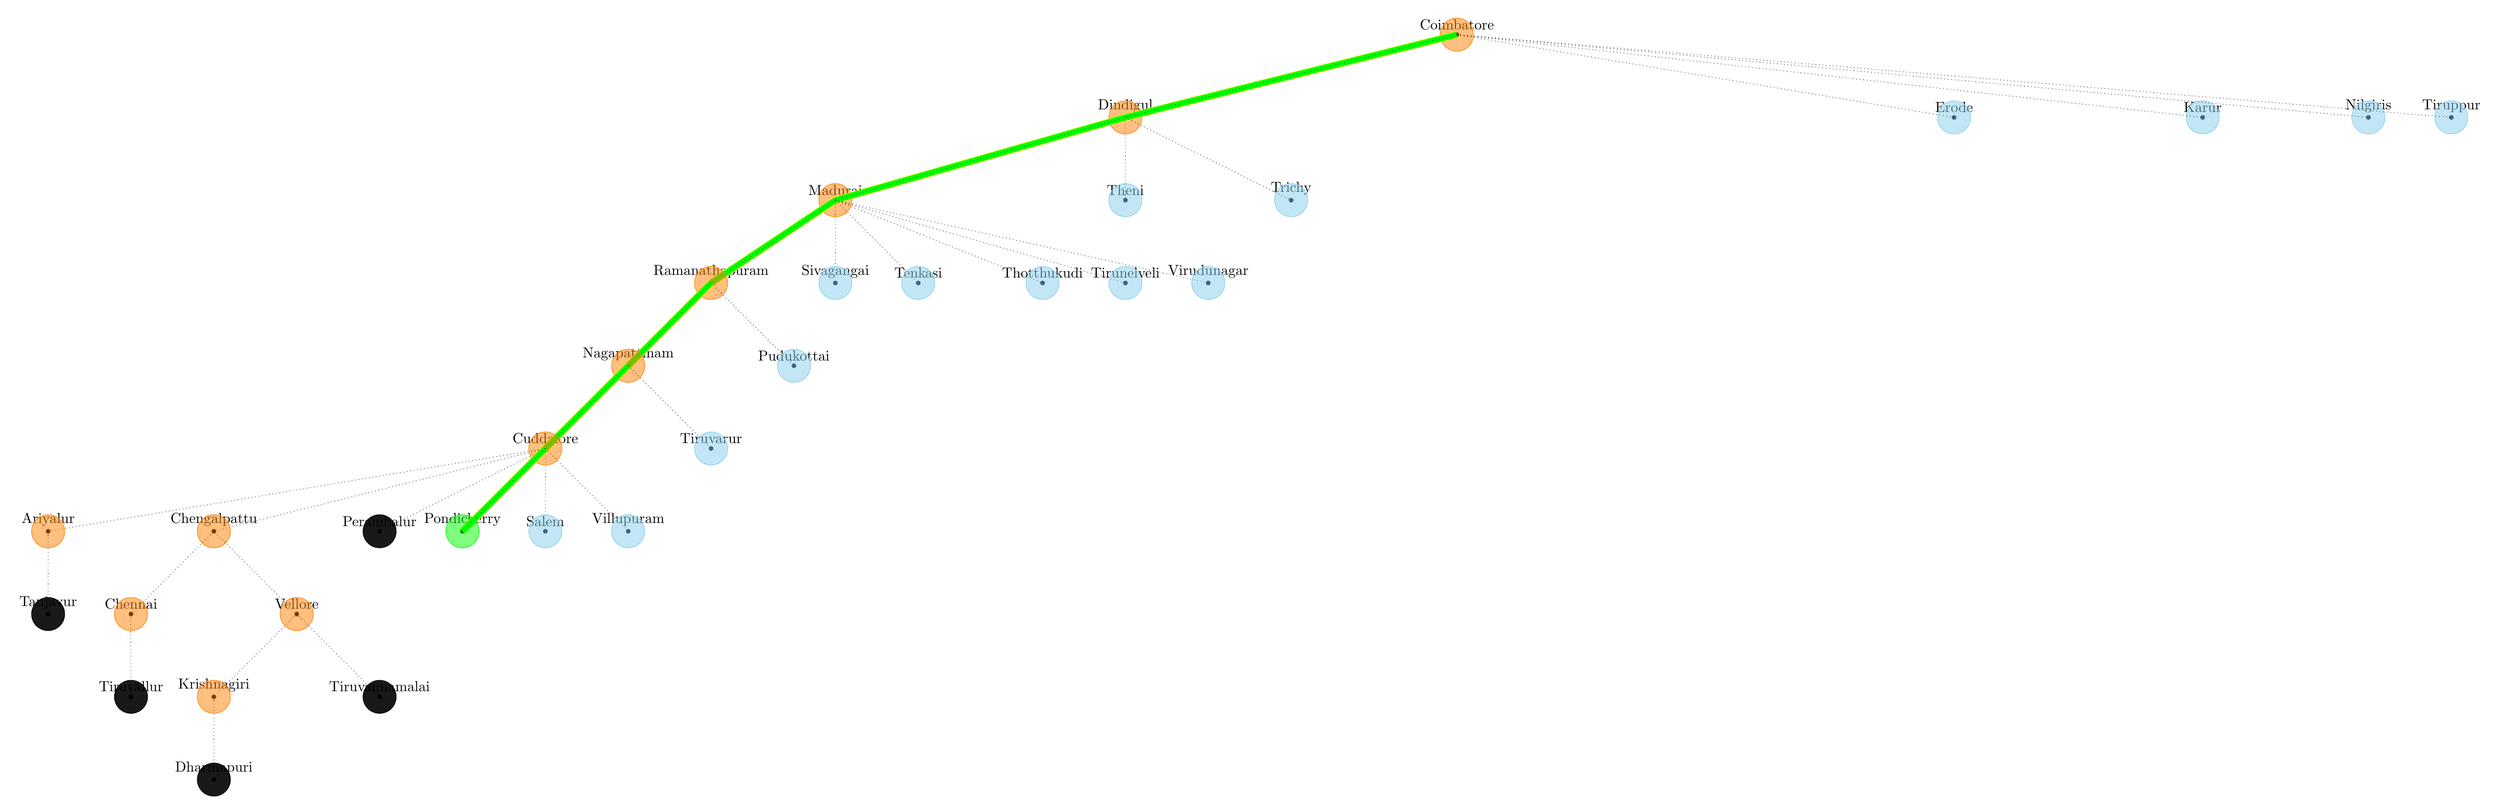
\begin{tikzpicture}
    \draw [black, fill=black ] (-18,0) circle [radius=0.05] node[above] {Coimbatore};
    \drawMineVisited{(-18,0)};

    %for coimbatore
    \draw [fill=black] (-26,-2) circle [radius=0.05] node[above] {Dindigul};
    \drawMineVisited{(-26,-2)};
    \draw [ dotted, preaction={%But before that
    draw,yellow,-,% Draw yellow without any arrow head
    double=green,
    double distance=10\pgflinewidth,
    }] (-18,0) -- (-26,-2);

    \draw [fill=black] (-6,-2) circle [radius=0.05] node[above] {Erode};
    \drawMineFrontier{(-6,-2)};
    \draw [ dotted] (-18,0) -- (-6,-2);

    \draw [fill=black] (0,-2) circle [radius=0.05] node[above] {Karur};
	\drawMineFrontier{(-0,-2)};
    \draw [ dotted] (-18,0) -- (-0,-2);

    \draw [fill=black] (4,-2) circle [radius=0.05] node[above] {Nilgiris};
	\drawMineFrontier{(4,-2)};
    \draw [ dotted] (-18,0) -- (4,-2);

    \draw [fill=black] (6,-2) circle [radius=0.05] node[above] {Tiruppur};
	\drawMineFrontier{(6,-2)};
    \draw [ dotted] (-18,0) -- (6,-2);

    %for dindigul
    % \draw [fill=black] (-25,-4) circle [radius=0.05] node[above] {Coimbatore};
    % \draw [fill=black] (-22,-4) circle [radius=0.05] node[above] {Karur};
    \draw [fill=black] (-33,-4) circle [radius=0.05] node[above] {Madurai};
	\drawMineVisited{(-33,-4)};
    \draw [ dotted, preaction={%But before that
    draw,yellow,-,% Draw yellow without any arrow head
    double=green,
    double distance=10\pgflinewidth,
    }] (-26,-2) -- (-33,-4);

    \draw [fill=black] (-26,-4) circle [radius=0.05] node[above] {Theni};
	\drawMineFrontier{(-26,-4)};
    \draw [ dotted] (-26,-2) -- (-26,-4);
    
    \draw [fill=black] (-22,-4) circle [radius=0.05] node[above] {Trichy};
	\drawMineFrontier{(-22,-4)};
    \draw [ dotted] (-26,-2) -- (-22,-4);

    %for madurai
    \draw [fill=black] (-36,-6) circle [radius=0.05] node[above] {Ramanathapuram};
    \draw [ dotted, preaction={%But before that
    draw,yellow,-,% Draw yellow without any arrow head
    double=green,
    double distance=10\pgflinewidth,
    }] (-33,-4) -- (-36,-6);
    \drawMineVisited{(-36,-6)};

    \draw [fill=black] (-33,-6) circle [radius=0.05] node[above] {Sivagangai};
    \draw [ dotted] (-33,-4) -- (-33,-6);
    \drawMineFrontier{(-33,-6)};

    \draw [fill=black] (-31,-6) circle [radius=0.05] node[above] {Tenkasi};
    \draw [ dotted] (-33,-4) -- (-31,-6);
    \drawMineFrontier{(-31,-6)};

    \draw [fill=black] (-28,-6) circle [radius=0.05] node[above] {Thotthukudi};
    \draw [ dotted] (-33,-4) -- (-28,-6);
    \drawMineFrontier{(-28,-6)};

    \draw [fill=black] (-26,-6) circle [radius=0.05] node[above] {Tirunelveli};
    \draw [ dotted] (-33,-4) -- (-26,-6);
    \drawMineFrontier{(-26,-6)};

    \draw [fill=black] (-24,-6) circle [radius=0.05] node[above] {Virudunagar};
    \draw [ dotted] (-33,-4) -- (-24,-6);
    \drawMineFrontier{(-24,-6)};

    %for Ramanathapuram
    \draw [fill=black] (-34,-8) circle [radius=0.05] node[above] {Pudukottai};
    \draw [ dotted] (-36,-6) -- (-34,-8);
    \drawMineFrontier{(-34,-8)};

    \draw [fill=black] (-38,-8) circle [radius=0.05] node[above] {Nagapattinam};
    \draw [ dotted, preaction={%But before that
    draw,yellow,-,% Draw yellow without any arrow head
    double=green,
    double distance=10\pgflinewidth,
    }] (-36,-6) -- (-38,-8);
    \drawMineVisited{(-38,-8)};
    %for  Sivagangai


    %for Nagapattinam
    \draw [fill=black] (-40,-10) circle [radius=0.05] node[above] {Cuddalore};
    \draw [ dotted, preaction={%But before that
    draw,yellow,-,% Draw yellow without any arrow head
    double=green,
    double distance=10\pgflinewidth,
    }] (-38,-8) -- (-40,-10);
    \drawMineVisited{(-40,-10)};

    \draw [fill=black] (-36,-10)  circle [radius=0.05] node[above] {Tiruvarur};
    \draw [ dotted] (-38,-8) -- (-36,-10) ;
    \drawMineFrontier{(-36,-10) };

    %for Cuddalore
    \draw [fill=black] (-52,-12) circle [radius=0.05] node[above] {Ariyalur};
    \draw [ dotted] (-40,-10)-- (-52,-12);
    \drawMineVisited{(-52,-12)};

    \draw [fill=black] (-48,-12) circle [radius=0.05] node[above] {Chengalpattu};
    \draw [ dotted] (-40,-10)-- (-48,-12);
    \drawMineVisited{(-48,-12)};

    \draw [fill=black] (-44,-12) circle [radius=0.05] node[above] {Perambalur};
    \draw [ dotted] (-40,-10)-- (-44,-12);
    \drawMineNotFound{(-44,-12)};

    \draw [fill=black] (-42,-12) circle [radius=0.05] node[above] {Pondicherry};
    \draw [ dotted, preaction={%But before that
    draw,yellow,-,% Draw yellow without any arrow head
    double=green,
    double distance=10\pgflinewidth,
    }] (-40,-10)-- (-42,-12);
    \drawMineFound{(-42,-12)};

    \draw [fill=black] (-40,-12) circle [radius=0.05] node[above] {Salem};
    \draw [ dotted] (-40,-10)-- (-40,-12);
    \drawMineFrontier{(-40,-12)};

    \draw [fill=black] (-38,-12) circle [radius=0.05] node[above] {Villupuram};
    \draw [ dotted] (-40,-10)-- (-38,-12);
    \drawMineFrontier{(-38,-12)};

    %for Ariyalur
    \draw [fill=black] (-52,-14) circle [radius=0.05] node[above] {Tanjavur};
    \draw [ dotted] (-52,-12)-- (-52,-14);
    \drawMineNotFound{(-52,-14)};
    
    % for Chengalpattu
    \draw [fill=black] (-50,-14) circle [radius=0.05] node[above] {Chennai};
    \draw [ dotted] (-50,-14)-- (-48,-12);
    \drawMineVisited{(-50,-14)};

    \draw [fill=black] (-46,-14) circle [radius=0.05] node[above] {Vellore};
    \draw [ dotted] (-46,-14)-- (-48,-12);
    \drawMineVisited{(-46,-14)};

    % for chennai
    \draw [fill=black] (-50,-16) circle [radius=0.05] node[above] {Tiruvallur};
    \draw [ dotted] (-50,-14)-- (-50,-16);
    \drawMineNotFound{(-50,-16)};

    % for vellore
    \draw [fill=black] (-48,-16) circle [radius=0.05] node[above] {Krishnagiri};
    \draw [ dotted] (-46,-14)-- (-48,-16);
    \drawMineVisited{(-48,-16)};

    \draw [fill=black] (-44,-16) circle [radius=0.05] node[above] {Tiruvannamalai};
    \draw [ dotted] (-46,-14)-- (-44,-16);
    \drawMineNotFound{(-44,-16)};

    %for Krishnagiri
    \draw [fill=black] (-48,-18) circle [radius=0.05] node[above] {Dharmapuri};
    \draw [ dotted] (-48,-16)--(-48,-18);
    \drawMineNotFound{(-48,-18)};

\end{tikzpicture}
\end{document}


